\documentclass[10pt,t]{beamer}


\setbeamersize{text margin left=10pt,text margin right=10pt}
\usetheme{lehigh}

\usefonttheme{professionalfonts}
\usefonttheme{serif}

%\usepackage{pgf,pgfarrows,pgfnodes,pgfautomata,pgfheaps,pgfshade}
%\usepackage{amsmath,amssymb,amsfonts,subfigure,pifont}
\usepackage{multirow,multicol}
%\usepackage{tabularx}
%\usepackage{booktabs}
\usepackage{colortbl}
\usepackage{algorithm,algpseudocode}
%\usepackage{etex}
\usepackage{fancyvrb,listings}

\definecolor{dkgreen}{rgb}{0,0.6,0}
\definecolor{grey}{rgb}{0.5,0.5,0.5}
\definecolor{mauve}{rgb}{0.58,0,0.82} 
\lstset{%
language=bash,                % the language of the code
%basicstyle=\footnotesize,           % the size of the fonts that are used for the code
basicstyle=\fontsize{4.5}{5.5}\selectfont\ttfamily,
showspaces=false,               % show spaces adding particular underscores
showstringspaces=false,         % underline spaces within strings
showtabs=false,                 % show tabs within strings adding particular underscores
%frame=single,                   % adds a frame around the code
%rulecolor=\color{black},        % if not set, the frame-color may be changed on line-breaks within not-black text (e.g. comments (green here))
tabsize=2,                      % sets default tabsize to 2 spaces
%captionpos=b,                   % sets the caption-position to bottom
breaklines=true,                % sets automatic line breaking
breakatwhitespace=false,        % sets if automatic breaks should only happen at whitespace
%title=\lstname,                   % show the filename of files included with \lstinputlisting;
% also try caption instead of title
keywordstyle=\color{blue},          % keyword style
commentstyle=\color{dkgreen},       % comment style
stringstyle=\color{mauve},         % string literal style
escapeinside={\%*}{*)},            % if you want to add LaTeX within your code
morekeywords={*,\dots,elif},              % if you want to add more keywords to the set
deletekeywords={\dots},              % if you want to delete keywords from the given language
%morecomment=[l]{//}
}
\lstset{%
language=csh,                % the language of the code
%basicstyle=\footnotesize,           % the size of the fonts that are used for the code
basicstyle=\fontsize{4.5}{5.5}\selectfont\ttfamily,
showspaces=false,               % show spaces adding particular underscores
showstringspaces=false,         % underline spaces within strings
showtabs=false,                 % show tabs within strings adding particular underscores
%frame=single,                   % adds a frame around the code
%rulecolor=\color{black},        % if not set, the frame-color may be changed on line-breaks within not-black text (e.g. comments (green here))
tabsize=2,                      % sets default tabsize to 2 spaces
captionpos=b,                   % sets the caption-position to bottom
breaklines=true,                % sets automatic line breaking
breakatwhitespace=false,        % sets if automatic breaks should only happen at whitespace
%title=\lstname,                   % show the filename of files included with \lstinputlisting;
% also try caption instead of title
keywordstyle=\color{blue},          % keyword style
commentstyle=\color{dkgreen},       % comment style
stringstyle=\color{mauve},         % string literal style
escapeinside={\%*}{*)},            % if you want to add LaTeX within your code
morekeywords={*,\dots,elif},              % if you want to add more keywords to the set
deletekeywords={\dots},              % if you want to delete keywords from the given language
%morecomment=[l]{//}
}
\lstdefinestyle{LINUX}
{
%    backgroundcolor=\color{black},
    basicstyle=\tiny\ttfamily,
%    keywordsstyle=\color{blue},
%    morekeywords={Tutorials,BASH,scripts},
%    literate={>}{{\textcolor{blue}{>}}}1
%         {/}{{\textcolor{blue}{/}}}1
%         {./}{{\textcolor{black}{./ }}}1
%         {~}{{\textcolor{blue}{\textasciitilde}}}1,
}

\lstdefinestyle{customc}{
  belowcaptionskip=1\baselineskip,
  breaklines=true,
  xleftmargin=\parindent,
  language=C,
  showstringspaces=false,
  basicstyle=\footnotesize\ttfamily,
  keywordstyle=\bfseries\color{green!40!black},
  commentstyle=\upshape\color{red!90!white},
  identifierstyle=\color{blue},
  stringstyle=\color{orange},
}
\lstdefinelanguage{OmpFortran}[]{Fortran}{
   rulesepcolor=\color{black},
   %
   extendedchars=true,
   %
   morecomment=[l] [\bfseries\color{red!90!white}]{!\$omp},
   morecomment=[l] [\bfseries\color{red!90!white}]{c\$omp},
   morecomment=[l] [\bfseries\color{red!90!white}]{*\$omp},
   morecomment=[l] [\bfseries\color{red!90!white}]{!\$acc},
   morecomment=[l] [\bfseries\color{red!90!white}]{c\$acc},
   morecomment=[l] [\bfseries\color{red!90!white}]{*\$acc},
}[comments]

\lstdefinelanguage{OmpC}[]{OmpFortran}{
   rulesepcolor=\color{black},
   %
   extendedchars=true,
   %
   morecomment=[l] [\bfseries\color{red!90!white}]{\#pragma\ omp},
   morecomment=[l] [\bfseries\color{red!90!white}]{\#pragma\ acc},
}[comments]

\lstset{escapechar=@,style=customc}
\lstset{literate=%
   *{0}{{{\color{blue}0}}}1
    {1}{{{\color{blue}1}}}1
    {2}{{{\color{blue}2}}}1
    {3}{{{\color{blue}3}}}1
    {4}{{{\color{blue}4}}}1
    {5}{{{\color{blue}5}}}1
    {6}{{{\color{blue}6}}}1
    {7}{{{\color{blue}7}}}1
    {8}{{{\color{blue}8}}}1
    {9}{{{\color{blue}9}}}1
}

\algrenewcommand\algorithmicfunction{\textbf{program}}
\algblockdefx[Program]{Program}{EndProgram}[1]{\textbf{program} \textsc{#1}}[1]{\textbf{end program} \textsc{#1}}
\algloopdefx[doloop]{Do}[1]{\textbf{do} #1}
\algcblockdefx[doloop]{If}{Do}{EndDo}
[1]{\textbf{do} #1}{\textbf{end do}}


\usepackage{tikz}
\usetikzlibrary{shapes,arrows,matrix}
\usetikzlibrary{calc}
\pgfdeclarelayer{background}
\pgfdeclarelayer{foreground}
\pgfsetlayers{background,main,foreground}
\usepackage[latin1]{inputenc}
\usepackage[english]{babel}
\usepackage{hyperref}
\usepackage[normalem]{ulem}
% \usepackage{movie15} 

                                                         
\usepackage{times}
\usepackage[T1]{fontenc}
\usepackage{graphicx}


\definecolor{DarkGreen}{rgb}{0.0,0.3,0.0}
\definecolor{Blue}{rgb}{0.0,0.0,0.8} 
\definecolor{dodgerblue}{rgb}{0.1,0.1,1.0}
\definecolor{indigo}{rgb}{0.41,0.1,0.0}
\definecolor{seagreen}{rgb}{0.1,1.0,0.1}
\DeclareSymbolFont{extraup}{U}{zavm}{m}{n}
%\DeclareMathSymbol{\vardiamond}{\mathalpha}{extraup}{87}
\newcommand{\cmark}{\ding{51}}
\newcommand{\xmark}{\ding{55}}
\newcommand{\smark}{\ding{77}}
\newcommand*\vardiamond{\textcolor{lubrown}{%
  \ensuremath{\blacklozenge}}}
\newcommand*\up{\textcolor{green}{%
  \ensuremath{\blacktriangle}}}
\newcommand*\down{\textcolor{red}{%
  \ensuremath{\blacktriangledown}}}
\newcommand*\const{\textcolor{darkgray}%
  {\textbf{--}}}
\newcommand*\enter{\tikz[baseline=-0.5ex] \draw[<-] (0,0) -| (0.5,0.1);}
\newcommand{\bftt}[1]{\textbf{\texttt{#1}}}
\newcommand{\lstfortran}[1]{\lstinline[language={[90]Fortran},basicstyle=\footnotesize\ttfamily]|#1|}
\newcommand{\Verblue}[1]{\Verb[formatcom=\color{blue},commandchars=\\\{\}]!#1!}
\newcommand{\Verbindigo}[1]{\Verb[formatcom=\color{indigo},commandchars=\\\{\}]!#1!}

\setbeamercolor{uppercol}{fg=white,bg=red!30!black}%
\setbeamercolor{lowercol}{fg=black,bg=red!15!white}%
\setbeamercolor{uppercol1}{fg=white,bg=blue!30!black}%
\setbeamercolor{lowercol1}{fg=black,bg=blue!15!white}%%
\setbeamercolor{uppercol2}{fg=white,bg=green!30!black}%
\setbeamercolor{lowercol2}{fg=black,bg=green!15!white}%
\newenvironment{colorblock}[4]
{
\setbeamercolor{upperblock}{fg=#1,bg=#2}
\setbeamercolor{lowerblock}{fg=#3,bg=#4}
\begin{beamerboxesrounded}[upper=upperblock,lower=lowerblock,shadow=true]}
{\end{beamerboxesrounded}}
\newenvironment{ablock}[0]
{
\begin{beamerboxesrounded}[upper=uppercol,lower=lowercol,shadow=true]}
{\end{beamerboxesrounded}}
\newenvironment{bblock}[0]
{
\begin{beamerboxesrounded}[upper=uppercol1,lower=lowercol1,shadow=true]}
{\end{beamerboxesrounded}}
\newenvironment{eblock}[0]
{
\begin{beamerboxesrounded}[upper=uppercol2,lower=lowercol2,shadow=true]}
{\end{beamerboxesrounded}}


\beamertemplateballitem

\newcolumntype{a}{>{\columncolor{lulime}}c}
\newcolumntype{b}{>{\columncolor{lulime!60}}c}
\newcolumntype{f}{>{\columncolor{lulime!60}}l}


\hypersetup{
  pdftitle={C Programming}
  pdfauthor={Alexander B. Pacheco, LTS Research Computing, Lehigh University}
}

\title[C]{Introduction to C Programming}
\author[Alex Pacheco]{\large{Alexander~B.~Pacheco}}
\institute[Research Computing]{\href{http://researchcomputing.lehigh.edu}{Research Computing}\\Lehigh University}
\date{}%June 3, 2015}
     
\subject{Talks}
\keywords{Lehigh Research Computing Resources, C Programming}
% This is only inserted into the PDF information catalog. Can be left
% out. 


% Delete this, if you do not want the table of contents to pop up at
% the beginning of each subsection:
\AtBeginSection[]
{
  \begingroup
  \setbeamertemplate{background canvas}[vertical shading][bottom=lubrown,top=lubrown]
  \setbeamertemplate{footline}[myfootline] 
  \setbeamertemplate{section page}[mysection]
  \frame[c]{
    \sectionpage
  }
  \endgroup
%  \begin{frame}{Outline}
%    \tableofcontents
%  \end{frame}
}

%\titlegraphic{\includegraphics[scale=0.5]{lu}}

\begin{document}

\frame{\titlepage}

\begin{frame}{Outline}
  \tableofcontents
\end{frame}


\section{Introduction}
\begin{frame}{What is the C Language?}
  \begin{itemize}
    \item A general-purpose, procedural, imperative computer programming language.
    \item Developed in 1972 by Dennis M. Ritchie at the Bell Telephone Laboratories to develop the UNIX operating system.
    \item The UNIX operating system, the C compiler, and essentially all UNIX applications programs have been written in C.
    \item C is the most widely used computer language.
    \begin{itemize}
      \item Easy to learn
      \item Structured language
      \item Produces efficient programs
      \item Handles low-level activities
      \item Can be compiled on a variety of computer plaforms
    \end{itemize}
    \item Most of the state-of-the-art softwares have been implemented using C.
    \item Today's most popular Linux OS and RBDMS MySQL have been written in C.
  \end{itemize}
\end{frame}

\begin{frame}{What do you need to learn C?}
  \begin{enumerate}
    \item {C Compiler}
      \begin{itemize}
        \item What is a Compiler?
          \begin{itemize}
            \item A compiler is a computer program (or set of programs) that transforms source code written in a programming language (the source language) into another computer language (the target language, often having a binary form known as object code).
          \end{itemize}
        \item How does a compiler do?
          \begin{itemize}
            \item Translate C source code into a binary executable
          \end{itemize}
        \item List of Common Compilers:
          \begin{itemize}
            \item GCC GNU Project (Free, available on most *NIX systems)
            \item Intel Compiler
            \item NVIDIA HPC SDK (formerly Portland Group (PGI) Compiler)
            \item Microsoft Visual Studio
          \end{itemize}
      \end{itemize}
    \item {Text Editor}
      \begin{itemize}
        \item Emacs
        \item VI/VIM
        \item Notepad++ (avoid Notepad if you will eventually use a *NIX system)
        \item Integrated Development Environment: Eclipse, XCode, Visual Studio, etc
      \end{itemize}
  \end{enumerate}
\end{frame}

\section{Basics}
\begin{frame}[fragile]{Program Structure}
A C Program consists of the following parts
  \begin{itemize}
    \item Preprocessor Commands
    \item Functions
    \item Variables
    \item Statements \& Expressions
    \item Comments
  \end{itemize}
  \begin{columns}
    \column{0.5\textwidth}
    A Simple Hello World Code
    \lstinputlisting[language=C,basicstyle=\scriptsize\ttfamily]{./Example/hello.c}
    \column{0.5\textwidth}
    Compile and execute the code
    \begin{lstlisting}[style=LINUX]
dyn100077:Exercise apacheco$ gcc hello.c 
dyn100077:Exercise apacheco$ ./a.out 
Hello World!
    \end{lstlisting}
  \end{columns}
\end{frame}

\begin{frame}[fragile]{My First C Code}
  \lstinputlisting[language=C,numbers=left,basicstyle=\scriptsize\ttfamily]{./Example/hello.c}
  \begin{itemize}
    \item \lstinline[language=C,basicstyle=\scriptsize\ttfamily]|#include <stdio.h>| is a preprocessor command.
    \item[] It tells a C compiler to include stdio.h file before going to actual compilation.
    \item \lstinline[language=C,basicstyle=\scriptsize\ttfamily]|int main()| is the main function where program execution begins.
    \item \lstinline[language=C,basicstyle=\scriptsize\ttfamily]|/* ... */| is a comment and ignored by the compiler.
    \item \lstinline[language=C,basicstyle=\scriptsize\ttfamily]|printf(...)| is function that prints \lstinline[language=C,basicstyle=\scriptsize\ttfamily]|Hello World!| to the screen.
    \item \lstinline[language=C,basicstyle=\scriptsize\ttfamily]|return 0;| terminates main() function and returns the value 0.
  \end{itemize}
\end{frame}

%\section{Basic Syntax}
\begin{frame}[fragile,allowframebreaks]{Basic C Syntax}
  \begin{itemize}
  \item C is a case sensitive programming language i.e. program is not the same as Program or PROGRAM.
  \item Each individual statement must end with a semicolon. 
  \item Whitespace i.e. tabs or spaces is insignificant except whitespace within a character string.
  \item All C statments are free format i.e. no specified layout or column assignment as in FORTRAN77.
    \begin{lstlisting}[basicstyle=\scriptsize\ttfamily]
#include <stdio.h>
int main () {  /* My First C Code */  printf("Hello World!\n");  return 0;}
    \end{lstlisting}
  \item[] will produce the exact same result as the code on the previous slide.
  \item In C everything within \lstinline[basicstyle=\scriptsize\ttfamily]|/* and */| is a comment. Comments can span multiple lines.
    \begin{lstlisting}[basicstyle=\scriptsize\ttfamily]
/* this is single line comment */
/* This
is a 
multiline comment */
    \end{lstlisting}
  \item Always use proper comments in your code. Your code will most likely be handed to someone long after you are gone.
  \item Comments are completely ignored by compiler (test/debug code)
  \end{itemize}
\end{frame}

\begin{frame}[fragile]{Valid Character Set in C language}
  \begin{center}
    \vspace{-0.5cm}
    \begin{tabular}{ab}
%      \hline
      {Alphabets} & ABCDEFGHIJKLMNOPQRSTUVWXYZ \\
      & abcdefghijklmnopqrstuvwxyz \\
      Digits                     & 0123456789 \\
%      \hline
    \end{tabular}
    \vspace{0.25cm}
    \newline
    \begin{tabular}{abababababababa}
%      \hline
      \rowcolor{lublue}\multicolumn{15}{a}{Special Characters} \\
%      \hline
      , & \_ & \{ & < & ' & ( & \Verb|^| & ; & \$ & / & *                & + & [ & \Verb|#| & ? \\ 
      . & \& & \} & > & " & ) & \Verb|!| & : & \% & | & \textbackslash{} & - & ] & \Verb|~| & \\
%      \hline
    \end{tabular}
    \vspace{0.25cm}
    \newline
    \begin{tabular}{cccc}
%      \hline
      \rowcolor{lublue}\multicolumn{4}{a}{Reserved Keywords}\\
%      \hline
      \rowcolor{lulime!60} auto     & double & int      & struct \\
      \rowcolor{lulime}    break    & else   & long     & switch \\
      \rowcolor{lulime!60} case     & enum   & register & typedef \\
      \rowcolor{lulime}    char     & extern & return   & union \\
      \rowcolor{lulime!60} continue & for    & signed   & void \\
      \rowcolor{lulime}    do       & if     & static   & while \\
      \rowcolor{lulime!60} default  & goto   & sizeof   & volatile \\
      \rowcolor{lulime}    const    & float  & short    & unsigned \\
%      \hline
    \end{tabular}
  \end{center}
  \begin{itemize}
    \item White space Characters: blank space, new line, horizontal tab, carriage return and form feed
  \end{itemize}
\end{frame}

%\section{Data Types, Variables, Constants and Operators}
\begin{frame}{Data Types}
  \begin{description}
    \item[Basic Types:] There are five basic data types
      \begin{enumerate}
        \item int - integer: a whole number.
        \item float - floating point value: ie a number with a fractional part.
        \item double - a double-precision floating point value.
        \item char -  a single character.
        \item void - valueless special purpose type.
      \end{enumerate}
    \item[Derived Types:] These include
      \begin{enumerate}
        \item Pointers
        \item Arrays
        \item Structures
        \item Union
        \item Function
      \end{enumerate}
  \end{description}
  \begin{itemize}
    \item The array and structure types are referred to collectively as the aggregate types. 
    \item The type of a function specifies the type of the function's return value.
  \end{itemize}
\end{frame}

\begin{frame}[fragile]{Basic Data Types: Integer}
  \begin{center}
    \begin{tabular}{ccc}
%      \hline
      \rowcolor{lublue}Type & Storage size (in bytes) & Value range \\
%      \hline
      \rowcolor{lulime}char            & 1      & -128 to 127 or 0 to 255 \\
      \rowcolor{lulime}unsigned char   & 1      & 0 to 255 \\
      \rowcolor{lulime}signed char     & 1      & -128 to 127 \\
%      \hline
      \rowcolor{lulime!60}\multirow{3}{*}{int} & 2 & -32,768 to 32,767 \\ \rowcolor{lulime!60}int & or & or \\ \rowcolor{lulime!60}& 4 &  -2,147,483,648 to 2,147,483,647 \\
%      \hline
      \rowcolor{lulime}\multirow{3}{*}{unsigned int} & 2 & 0 to 65,535 \\ \rowcolor{lulime}unsigned int& or & or  \\ \rowcolor{lulime}& 4 & 0 to 4,294,967,295 \\
%      \hline
      \rowcolor{lulime!60}short           & 2      & -32,768 to 32,767 \\
      \rowcolor{lulime!60}unsigned short  & 2      & 0 to 65,535 \\ 
%      \hline
      \rowcolor{lulime}long            & 4      & -2,147,483,648 to 2,147,483,647 \\
      \rowcolor{lulime}unsigned long   & 4      & 0 to 4,294,967,295 \\
%      \hline
    \end{tabular}
  \end{center}
  \begin{itemize}
    \item To get the exact size of a type or a variable on a particular platform, you can use the sizeof operator. 
    \item The expressions \lstinline[basicstyle=\scriptsize\ttfamily]|sizeof(type)| yields the storage size of the object or type in bytes. 
  \end{itemize}
\end{frame}

\begin{frame}{Basic Data Types: Floating-Point \& void}
  \begin{center}
    \begin{tabular}{abab}
%      \hline
      \rowcolor{lublue}Type & Storage size & Value range & Precision (decimal places) \\
%      \hline
      float       & 4 bytes  & 1.2E-38 to 3.4E38     & 6 \\
      double      & 8 bytes  & 2.3E-308 to 1.7E308   & 15 \\
      long double & 10 bytes & 3.4E-4932 to 1.1E4932 & 19 \\
%      \hline
    \end{tabular}
  \end{center}

  \begin{center}
    \begin{tabular}{ab}
%      \hline
      \rowcolor{lublue}Situation & Description \\
%      \hline
      function returns as void & function with no return value \\
      function arguments as void & function with no parameter \\
      pointers to void & address of an object without type \\
%      \hline
    \end{tabular}
  \end{center}
\end{frame}

\begin{frame}[fragile]{Variables}
  \begin{itemize}
    \item Variables are memory location in computer's memory to store data.
    \item To indicate the memory location, each variable should be given a unique name called identifier. 
    \item Variable names are just the symbolic representation of a memory location.
    \item Rules for variable names:
    \begin{enumerate}
      \item Composed of letters (both uppercase and lowercase letters), digits and underscore '\_' only.
      \item The first letter of a variable should be either a letter or an underscore.
      \item There is no rule for the length of a variable name.
      \begin{itemize}
        \item Most likely your code will be used by someone else, so variable names should be meaningful and short as possible.
      \end{itemize}
    \end{enumerate}
    \begin{lstlisting}[language=C,basicstyle=\scriptsize\ttfamily]
int num;
float circle_area;
double _volume;
    \end{lstlisting}
    \item In C programming, you have to declare variable before using it in the program.
  \end{itemize}
\end{frame}

\begin{frame}[fragile]{Declaring Variable or Variable Definition}
  \begin{itemize}
    \item A variable definition means to tell the compiler where and how much to create the storage for the variable. 
    \item A variable definition specifies a data type and contains a list of one or more variables of that type as follows:
    \item[] \lstinline[basicstyle=\scriptsize\ttfamily]{type variable_list;}
    \item \lstinline[basicstyle=\scriptsize\ttfamily]{type} must be a valid C data type or any user-defined object, etc., and 
    \item[] \lstinline[basicstyle=\scriptsize\ttfamily]{variable_list} may consist of one or more identifier names separated by commas.
    \item Variables can be initialized (assigned an initial value) in their declaration.
    \item[] \lstinline[basicstyle=\scriptsize\ttfamily]{type variable_name = value;}
  \end{itemize}
  \begin{lstlisting}[language=C,basicstyle=\scriptsize\ttfamily]
int    i, j, k;
char   c, ch;
float  f, salary;
double d;
int d = 3, f = 5;           // definition and initializing d and f. 
byte z = 22;                // definition and initializes z. 
char x = 'x';               // the variable x has the value 'x'.
  \end{lstlisting}
\end{frame}

\begin{frame}{Constants \& Literals}
  The constants refer to fixed values that the program may not alter during its execution. These fixed values are also called literals.
  {\footnotesize
    \begin{columns}
      \column{0.45\textwidth}
      \begin{block}{Integer Constants}
        \begin{tabular}{ll}
          85         & /* decimal */\\
          0213       & /* octal */\\
          0x4b       & /* hexadecimal */\\
          30         & /* int */\\
          30u        & /* unsigned int */\\
          30l        & /* long */\\
          30ul       & /* unsigned long */\\
        \end{tabular}
      \end{block}
      \begin{block}{Character Constants}
        \begin{tabular}{ll}
          'a'                               & /* character 'a' */\\
          'Z'                               & /* character 'Z' */\\
          \textbackslash?                   & /*? character */\\
          \textbackslash{}\textbackslash{}  & /*\textbackslash{} character */\\
          \textbackslash{}n                 & /*Newline */\\
          \textbackslash{}r                 & /*Carriage return */\\
          \textbackslash{}t                 & /*Horizontal tab */\\
        \end{tabular}
      \end{block}
      \column{0.45\textwidth}
      \begin{block}{Floating Point Constants}
        \begin{tabular}{ll}
          3.1416    & \\
          314159E-5 & /* 3.14159 */\\
          2.1E+5    & /* 2.1x$10^5$*/\\
          3.7E-2    & /* 0.037 */\\
          0.5E7     & /* 5.0x$10^6$*/\\
          -2.8E-2   & /* -0.028 */\\
        \end{tabular}
      \end{block}
        \begin{block}{String Constants}
          \begin{tabular}{ll}
            "hello, world"  & /* normal string */\\
            "c programming \textbackslash{} & \multirow{2}{*}{/* multi-line string */}\\
            language" & \\
          \end{tabular}
      \end{block}
    \end{columns}
  }
\end{frame}

\begin{frame}[fragile]{How to define Constants}
  \begin{itemize}
    \item Constants can be defined in two ways
    \begin{enumerate}
      \item Using the \lstinline[language=C,basicstyle=\scriptsize\ttfamily]{#define} preprocessor (defining a macro)
      \item Using the \lstinline[language=C,basicstyle=\scriptsize\ttfamily]{const} keyword (new standard borrowed from C++)
    \end{enumerate}
  \end{itemize}
  \lstinputlisting[language=C,basicstyle=\scriptsize\ttfamily]{./Example/const.c}
\end{frame}

\begin{frame}{Input and Output}
  \begin{itemize}
    \item C or any programming language in general needs to be interactive i.e. write something back and optionally read data to be useful.
    \item Similar to Unix, C treats all devices as files.
      \begin{center}
        \begin{tabular}{abb}
%          \hline
          \rowcolor{lublue}Standard File & File Pointer & Device \\
%          \hline
          Standard Input & stdin & Keyboard \\
          Standard Output & stdout & Screen \\
          Standard Error & stderr & Screen\\
%          \hline
        \end{tabular}
      \end{center}
      
    \item C Programming language provides three functions to read/write from standard input/output
      \begin{center}
        \begin{tabular}{cccc}
%          \hline
          \rowcolor{lublue}& \multicolumn{2}{c}{Unformatted} & Formatted \\
%          \hline
          \rowcolor{lulime}Input & getchar & gets & scanf \\
          \rowcolor{lulime!60}Output & putchar & puts & printf \\
%          \hline
        \end{tabular}
      \end{center}
  \end{itemize}
\end{frame}

\begin{frame}[fragile]{Unformatted I/O}
  \begin{block}{The getchar() \& putchar() functions}
    \begin{itemize}
      \item The \lstinline[language=C,basicstyle=\scriptsize\ttfamily]|int getchar(void)| function reads the next available character from the screen and returns it as an integer. 
      \item[] This function reads only single character at a time.
      \item The \lstinline[language=C,basicstyle=\scriptsize\ttfamily]|int putchar(int c)| function puts the passed character on the screen and returns the same character. 
      \item[] This function puts only single character at a time. 
    \end{itemize}
  \end{block}

  \begin{block}{The gets() \& puts() functions}
    \begin{itemize}
      \item The \lstinline[language=C,basicstyle=\scriptsize\ttfamily]|char *gets(char *s)| function reads a line from stdin into the buffer pointed to by s until either a terminating newline or EOF.
      \item The \lstinline[language=C,basicstyle=\scriptsize\ttfamily]|int puts(const char *s)| function writes the string s and a trailing newline to stdout.
    \end{itemize}
  \end{block}
\end{frame}

\begin{frame}[fragile]
  \begin{columns}
    \column{0.5\textwidth}
    \lstinputlisting[language=C,basicstyle=\scriptsize\ttfamily]{./Example/readiounfmt1.c}
    \column{0.5\textwidth}
    \lstinputlisting[language=C,basicstyle=\scriptsize\ttfamily]{./Example/readiounfmt2.c}
  \end{columns}
\end{frame}

\begin{frame}[fragile]{Formatted I/O}
  \begin{itemize}
    \item The \lstinline[language=C,basicstyle=\scriptsize\ttfamily]|int scanf(const char *format, ...)| function reads input from the standard input stream stdin and scans that input according to format provided.
    \item The \lstinline[language=C,basicstyle=\scriptsize\ttfamily]|int printf(const char *format, ...)| function writes output to the standard output stream stdout and produces output according to a format provided (optional).
      \lstinputlisting[language=C,basicstyle=\scriptsize\ttfamily]{./Example/helloworld.c}
    \item In this program, the user is asked a input and value is stored in variable \lstinline|name|.
    \item Note the '\lstinline[language=C,basicstyle=\scriptsize\ttfamily]|&|' sign before \lstinline[language=C,basicstyle=\scriptsize\ttfamily]|name|.
    \item \lstinline[language=C,basicstyle=\scriptsize\ttfamily]|&name| denotes the address of \lstinline[language=C,basicstyle=\scriptsize\ttfamily]|name| and value is stored in that address.
  \end{itemize}
\end{frame}

\begin{frame}[fragile]{Common Format Specifier}
  \begin{itemize}
    \item The format specifier: \lstinline[language=C,basicstyle=\footnotesize\ttfamily]|%[flags][width][.precision][length]specifier| 
  \end{itemize}
  \begin{center}
    \begin{tabular}{cl}
%      \hline
      \rowcolor{lublue}flag & meaning \\
%      \hline
      \rowcolor{lulime}- & left justify \\
      \rowcolor{lulime}+ & always display sign\\
      \rowcolor{lulime}0 & pad with leading zeros\\
%      \hline
    \end{tabular}
  \end{center}
  \begin{center}
    \begin{tabular}{ccc}
%      \hline
      \rowcolor{lublue}Specifier & Output & Example\\
%      \hline
      \rowcolor{lulime}\%f & decimal float & 3.456 \\
%      \hline
      \rowcolor{lulime!80}\%7.5f & decimal float, 7 digit width and 5 digit precision & 3.45600 \\
%      \hline
      \rowcolor{lulime}\%d & integer & 5\\
%      \hline
      \rowcolor{lulime!70}\%05d & integer, 5 digits pad with zeros & 00101 \\
%      \hline
      \rowcolor{lulime}\%s & string of characters & "Hello World!"\\
%      \hline
      \rowcolor{lulime!60}\%e & scientific notation for decimal float & 2.71828e+5  \\
%      \hline
      \rowcolor{lulime}\%c & character &  \\
%      \hline
      \rowcolor{lulime!50}\textbackslash{}n & insert new line & \\
%      \hline
      \rowcolor{lulime}\textbackslash{}t & insert tab & \\
%      \hline
    \end{tabular}
  \end{center}
\end{frame}

\begin{frame}[fragile]{}
  \lstinputlisting[language=C,basicstyle=\scriptsize\ttfamily]{./Example/print.c}
  \begin{lstlisting}[style=LINUX]
alexanders-mbp:Example apacheco$ gcc -o print print.c
alexanders-mbp:Example apacheco$ ./print
Characters: a A 
Decimals: 2014 0065
         floats: 3.14160        3.141600        3.141600e+00 
hello world 

  \end{lstlisting}
\end{frame}

%\section{Programming Operators}
\begin{frame}{Operators}
  \begin{itemize}
    \item Arithmetic
      \begin{center}
        \begin{tabular}{ab}
%          \hline
          \rowcolor{lublue}Operator & Meaning \\
%          \hline
          +  & addition or unary plus \\
          -  & subtraction or  unary minus \\
          *  & multiplication \\
          /  & division \\
          \% & remainder after division( modulo division) \\
          ++ & increase integer value by one \\
          {-}{-} & decrease integer value by one \\
%          \hline
        \end{tabular}
      \end{center}
      \item Assignment Operator
        \begin{center}
          \begin{tabular}{abb}
%            \hline
            \rowcolor{lublue}Operator & Example & Same as \\
%            \hline
            =   & a=b   & a=b \\
            +=  & a+=b  & a=a+b \\
            -=  & a-=b  & a=a-b \\
            *=  & a*=b  & a=a*b \\
            /=  & a/=b  & a=a/b \\
            \%= & a\%=b & a=a\%b \\
%            \hline
          \end{tabular}
        \end{center}
  \end{itemize}
\end{frame}

\begin{frame}[fragile]{Increment/Decrement Operator}
  \begin{itemize}
    \item There are two types of increment/decrement operators
    \begin{enumerate}
      \item Suffix or Postfix: e.g. i++ or j{-}{-}
      \item[] a=i++ means set a to i and then increment i by 1
      \item Prefix: ++i or {-}{-}j
      \item[] a=++i means increment i by 1 and then set a to i
    \end{enumerate}
    \item Consider the following example
    \item[] If i = 1 and j = 2, then
    \item[] ++i + j++ = 4
    \item[] and not 5 since j is incremented after the operation is complete
  \end{itemize}
  \begin{columns}
    \column{0.45\textwidth}
    \lstinputlisting[basicstyle=\tiny\ttfamily]{./Example/increment.c}
    \column{0.45\textwidth}
    \begin{lstlisting}[style=LINUX]
alexanders-mbp:Example apacheco$ make increment
cc     increment.c   -o increment
alexanders-mbp:Example apacheco$ ./increment
++i + j++: 4
a=++i: 2, b=j++: 2, i:2, j:3
a(=++i) + b(=j++): 4
    \end{lstlisting}
  \end{columns}
\end{frame}

\begin{frame}{Relational Operators}
  \begin{itemize}
  \item Relational operators checks relationship between two operands.
  \item If the relation is true, it returns value 1 and if the relation is false, it returns value 0.
  \item Relational operators are used in decision making and loops in C programming.
  \end{itemize}
  \begin{center}
    \begin{tabular}{abb}
%      \hline
      \rowcolor{lublue}Operator & Meaning & Example \\
%      \hline
      == & Equal to                 & 5==3 returns false (0) \\
      >  & Greater than             & 5>3 returns true (1) \\
      <  & Less than                & 5<3 returns false (0) \\
      != & Not equal to             & 5!=3 returns true(1) \\
      >= & Greater than or equal to & 5>=3 returns true (1) \\
      <= & Less than or equal to    & 5<=3 return false (0) \\
%      \hline
    \end{tabular}
  \end{center}
\end{frame}

\begin{frame}[fragile]{Logical \& Conditional Operators}
  \begin{itemize}
  \item Logical operators are used to combine expressions containing relation operators.
  \item In C, there are 3 logical operators
  \end{itemize}
  \begin{center}
    \begin{tabular}{abb}
%      \hline
      \rowcolor{lublue}Operator & Meaning & Example \\
%      \hline
      \&\& & Logial AND  & If c=5 and d=2 then,((c==5) \&\& (d>5)) returns false. \\
      ||   & Logical OR  & If c=5 and d=2 then, ((c==5) || (d>5)) returns true. \\
      !    & Logical NOT & If c=5 then, !(c==5) returns false. \\
%      \hline
    \end{tabular}
  \end{center}
  \begin{itemize}
  \item Conditional Operator: Conditional operators are used in decision making in C programming, i.e, executes different statements according to test condition whether it is either true or false.
  \item[] \lstinline[language=C,basicstyle=\scriptsize\ttfamily]|conditional_expression?expression1:expression2|
  \item If the test condition is true, expression1 is returned and if false expression2 is returned.
  \item[] \lstinline[language=C,basicstyle=\scriptsize\ttfamily]|d=(c>0)?10:-10;|
  \item[] If c is greater than 0, value of d will be 10 but, if c is less than 0, value of d will be -10.
  \end{itemize}
\end{frame}

\begin{frame}[fragile]{Other Operators}
  \begin{itemize}
  \item Bitwise Operators: works on bits and perform bit-by-bit operation
    \begin{tabular}{aabbb}
      \rowcolor{lublue}\multicolumn{5}{c}{Truth Table} \\
      \rowcolor{lublue}p & q & p \& q & p | q & p \Verb|^| q \\
      0 & 0 & 0 & 0 & 0 \\
      0 & 1 & 0 & 1 & 1 \\
      1 & 1 & 1 & 1 & 0 \\
      1 & 0 & 0 & 1 & 1 \\ 
    \end{tabular}
  \item Misc Operators
  \item[]
    \begin{tabular}{abb}
      \rowcolor{lublue}Operator & Description \\
      sizeof() & Returns the size of an variable. \\
      \& & Returns the address of an variable. \\
      * & Pointer to a variable. \\
      ? : & Conditional Expression \\
    \end{tabular}
  \end{itemize}
\end{frame}

\begin{frame}[fragile]{Operator Precedance}
  \scriptsize{
    \begin{center}
      \begin{tabular}{ccc}
        \hline
        \rowcolor{lublue}Operator & Description & Associativity \\
        \rowcolor{lulime!60}++, {-}{-} & Suffix Increment/Decrement & $\rightarrow$ \\
        \rowcolor{lulime}++, {-}{-} & Prefix Increment/Decrement & $\leftarrow$ \\
        \rowcolor{lulime!60}+, - & Unary plus and minus &  \\
        \rowcolor{lulime}!, \Verb|~| & Logical NOT and Bitwise NOT & \\
        \rowcolor{lulime!60}* & Indirection (dereference) & \\
        \rowcolor{lulime}\& & Address of & \\
        \rowcolor{lulime!60}sizeof & Size-of & \\
        \rowcolor{lulime}{*, /, \%} & Multiplication, division, modulo & $\rightarrow$ \\
        \rowcolor{lulime!60}{+, -} & Addition, Subtraction & \\
        \rowcolor{lulime}{<<, >>} & Bitwise left and right shift & \\
        \rowcolor{lulime!60}{<, <=} & Relational Operators & \\ 
        \rowcolor{lulime}{>, >= } &  & \\ 
        \rowcolor{lulime!60}{==, !=} &  & \\ 
        \rowcolor{lulime}{\&} & Bitwise AND & \\
        \rowcolor{lulime!60}{\Verb|^|} & Bitwise XOR & \\
        \rowcolor{lulime}{|} & Bitwise OR & \\
        \rowcolor{lulime!60}{\&\&} & Logical AND & \\
        \rowcolor{lulime}{||} & Logical OR & \\
        \rowcolor{lulime!60}{?:} & Ternary Conditional & $\leftarrow$ \\
        \rowcolor{lulime}{=} & Simple Assignment &  \\
        \rowcolor{lulime!60}{+=, -=} & Assignment by sum and difference & \\
        \rowcolor{lulime}{*=, /=, \%=} & Assignment by product, quotient and remainder & \\
        \rowcolor{lulime!60}{<<=, >>=} & Assignment by bitwise left and right shift & \\
        \rowcolor{lulime}{\&=, \Verb|^=|, |=} & Assignment by logical AND, XOR and OR & \\
        \rowcolor{lulime!60}{,} & Comma Operator & $\rightarrow$ \\
        \hline
      \end{tabular}
    \end{center}
  }
\end{frame}

\section{Control Flow}
\begin{frame}{Control Flow}
  \begin{itemize}
    \item Conditional Statements (decision making/selection)
    \begin{itemize}
      \item if $\cdots$ else if $\cdots$ else
      \item switch
    \end{itemize}
    \item Loops
    \begin{itemize}
      \item for
      \item while
      \item do while
    \end{itemize}
  \end{itemize}
\end{frame}

\begin{frame}[fragile]{if statement}
  \begin{itemize}
    \item An if statement consists of a boolean expression followed by one or more statements.
      \begin{lstlisting}[language=C,basicstyle=\scriptsize\ttfamily]
if(expression)
{
   /* statement(s) will execute if the boolean expression is true */
}
      \end{lstlisting}
    \item If the boolean expression evaluates to true, then the block of code inside the if statement will be executed. 
    \item If boolean expression evaluates to false, then the first set of code after the end of the if statement(after the closing curly brace) will be executed.
  \end{itemize}
\end{frame}

\begin{frame}[fragile]{if $\cdots$ else statement}
  \begin{itemize}
    \item An if statement can be followed by an optional else statement, which executes when the boolean expression is false.
      \begin{lstlisting}[language=C,basicstyle=\scriptsize\ttfamily]
if(expression)
{
   /* statement(s) will execute if the boolean expression is true */
}
else
{
  /* statement(s) will execute if the boolean expression is false */
}
      \end{lstlisting}
    \item If the boolean expression evaluates to true, then the if block of code will be executed, otherwise else block of code will be executed.
  \end{itemize}
\end{frame}

\begin{frame}[fragile]{if $\cdots$ else if $\cdots$ else statement}
  \begin{itemize}
    \item An if statement can be followed by an optional else if$\cdots$else statement,
    \item very useful to test various conditions using single if$\cdots$else if statement.
    \item When using if , else if , else statements there are few points to keep in mind:
    \begin{itemize}
      \item An if can have zero or one else's and it must come after any else if's.
      \item An if can have zero to many else if's and they must come before the else.
      \item Once an else if succeeds, none of the remaining else if's or else's will be tested.
    \end{itemize}
    \begin{lstlisting}[language=C,basicstyle=\scriptsize\ttfamily]
if(expression 1)
{
   /* Executes when the boolean expression 1 is true */
}
else if( expression 2)
{
   /* Executes when the boolean expression 2 is true */
}
else if( expression 3)
{
   /* Executes when the boolean expression 3 is true */
}
else 
{
   /* executes when the none of the above condition is true */
}
    \end{lstlisting}
  \end{itemize}
\end{frame}

\begin{frame}[fragile]{}
  \lstinputlisting[language=C,basicstyle=\scriptsize\ttfamily]{./Example/ifelseif.c}
\end{frame}

\begin{frame}[fragile]{Nested if$\cdots$else statement}
  \begin{itemize}
    \item You can use one if or else if statement inside another if or else if statement(s) i.e. nested if$\cdots$else statement/s
      \begin{lstlisting}[language=C,basicstyle=\scriptsize\ttfamily]
if( expression 1)
{
   /* Executes when the boolean expression 1 is true */
   if( expression 2)
   {
      /* Executes when the boolean expression 2 is true */
   }
}
      \end{lstlisting}
  \end{itemize}
\end{frame}

\begin{frame}[fragile]{}
  \lstinputlisting[language=C,basicstyle=\scriptsize\ttfamily]{./Example/nestedif.c}
\end{frame}

\begin{frame}[fragile,allowframebreaks]{switch statement}
  \begin{itemize}
    \item A switch statement allows a variable to be tested for equality against a list of values. 
    \item Each value is called a case, and the variable being switched on is checked for each switch case.
      \begin{lstlisting}[language=C,basicstyle=\scriptsize\ttfamily]
switch(expression){
    case constant-expression  :
       statement(s);
       break; /* optional */
    case constant-expression  :
       statement(s);
       break; /* optional */
  
    /* you can have any number of case statements */
    default : /* Optional */
       statement(s);
}
      \end{lstlisting}
    \item The expression used in a switch statement must have an integral type 
    \item[](or enumerated type, or be of a class type in which the class has a single conversion function to an integral or enumerated type).
    \item You can have any number of case statements within a switch. Each case is followed by the value to be compared to and a colon.
    \item The constant-expression for a case must be the same data type as the variable in the switch, and it must be a constant or a literal.
    \item When the variable being switched on is equal to a case, the statements following that case will execute until a break statement is reached.
    \item When a break statement is reached, the switch terminates, and the flow of control jumps to the next line following the switch statement.
    \item Not every case needs to contain a break. If no break appears, the flow of control will fall through to subsequent cases until a break is reached.
    \item A switch statement can have an optional default case, which must appear at the end of the switch. 
    \item The default case can be used for performing a task when none of the cases is true. No break is needed in the default case.
  \end{itemize}
  \lstinputlisting[language=C,basicstyle=\fontsize{5}{6}\ttfamily]{./Example/switch.c}
\end{frame}

\begin{frame}[fragile]{Nested Conditional Statements}
  \begin{itemize}
    \item Conditional statements can be nested as they do not overlap:
      \begin{lstlisting}[language=C,basicstyle=\scriptsize\ttfamily]
if( expression 1) {
  if(expression 2) {
    /* Executes when the boolean expression 2 is true */
    /* nested switch statement */
    switch(expression){
    case constant-expression :
      statement(s);
      break; /* optional */
    case constant-expression :
      statement(s);
      break; /* optional */
      /* you can have any number of case statements */
    default : /* Optional */
      statement(s);
    }
  }
 }
      \end{lstlisting}
  \end{itemize}
\end{frame}

\begin{frame}[fragile]{for loop}
  \begin{itemize}
    \item A for loop is a repetition control structure that allows you to efficiently write a loop that needs to execute a specific number of times.
      \begin{itemize}
        \item The init step is executed first and only once.
        \item the condition is evaluated. If it is true, the body of the loop is executed. If it is false, the body of the loop does not execute, the loop exits.
        \item the increment statement executes after the loop body.
        \item The loop continues until the condition becomes false
      \end{itemize}
      \begin{lstlisting}[language=C,basicstyle=\scriptsize\ttfamily]
for ( init; condition; increment )
{
   statement(s);
}
      \end{lstlisting}
  \end{itemize}
\end{frame}

\begin{frame}[fragile]{while and do$\cdots$while loops}
  \begin{itemize}
    \item while loops are similar to for loops
    \item A while loop continues executing the code block as long as the condition in the while holds.
      \begin{lstlisting}[language=C,basicstyle=\scriptsize\ttfamily]
while(condition)
{
   statement(s);
}
      \end{lstlisting}
    \item do$\cdots$while loop is guaranteed to execute at least one time.
      \begin{lstlisting}[language=C,basicstyle=\scriptsize\ttfamily]
do
{
   statement(s);

}while( condition );
      \end{lstlisting}
  \end{itemize}
\end{frame}

\begin{frame}[fragile]{Simple loops using for, while, do while}
  \lstinputlisting[language=C,basicstyle=\scriptsize\ttfamily]{./Example/loops.c}
\end{frame}

\begin{frame}[fragile]{Nested loops in C}
  \begin{itemize}
    \item All loops can be nested as long as they do not overlap
  \end{itemize}
  \begin{columns}
    \column{0.45\textwidth}
    \begin{lstlisting}[language=C,basicstyle=\scriptsize\ttfamily]
/* nested for loops*/
for (init; condition; increment) {
  for (init; condition; increment) {
    statement(s);
  }
  statement(s);
 }
/* nested while loops*/
while (condition) {
  while (condition) {
    statement(s);
  }
  statement(s);
 }
    \end{lstlisting}
    \column{0.45\textwidth}
    \begin{lstlisting}[language=C,basicstyle=\scriptsize\ttfamily]
/* nested do while loops*/
do {
  statement(s);
  do {
    statement(s);
  } while ( condition );
 } while ( condition );
/* mixed type loops*/
while (condition) {
  for (init; condition; increment) {
    statement(s);
    do {
      statement(s);
    } while ( condition );
  }
  statement(s);
 }
    \end{lstlisting}
  \end{columns}
\end{frame}

\begin{frame}[fragile]
  \lstinputlisting[language=C,basicstyle=\scriptsize\ttfamily]{./Example/nestedfor.c}
\end{frame}

\begin{frame}[fragile]{Loop Control Statement}
  \begin{itemize}
    \item Loop control statements change execution from its normal sequence.
      \begin{description}
        \item[break:] Terminates the loop or switch statement
        \item[continue:] Causes the loop to skip the remainder of its body for the current iteration
        \item[goto:] Transfers control to the labeled statement. Use is not advised
      \end{description}
  \end{itemize}
  \begin{columns}
    \column{0.45\textwidth}
    \lstinputlisting[language=C,basicstyle=\fontsize{5}{6}\selectfont\ttfamily]{./Example/break.c}
    \column{0.45\textwidth}
    \lstinputlisting[language=C,basicstyle=\fontsize{5}{6}\ttfamily]{./Example/continue.c}
  \end{columns}
\end{frame}

\section{Functions}
\begin{frame}[fragile]{Functions}
  \begin{itemize}
  \item A function is a group of statements that together perform a task.
  \item Every C program has at least one function, which is main()
  \item Functions receive either a fixed or variable amount of arguments.
  \item Functions can only return one value, or return no value (void).
  \item In C, arguments are \textbf{passed by value} to functions
  \item How to return value? - \textbf{Pointers}
  \item Functions are defined using the following syntax:
    \begin{lstlisting}[language=C,basicstyle=\scriptsize\ttfamily]
      return_type function_name( parameter list )
      {
        body of the function
      }
    \end{lstlisting}
  \item A function \textbf{declaration} tells the compiler about a function's name, return type, and parameters.
  \item A function \textbf{definition} provides the actual body of the function.
  \end{itemize}
\end{frame}

\begin{frame}[fragile]{Function Definition}
  \begin{itemize}
  \item \textbf{Return Type:} Function's return type is the data type of the value the function returns. When there is no return value, return void.
  \item \textbf{Function Name:} This is the actual name of the function.
  \item \textbf{Parameter:} The parameter list refers to the type, order, and number of the parameters of a function. A function may contain no parameters.
  \item \textbf{Function Body:} The function body contains a collection of statements that define the function behavior.
  \end{itemize}
  \lstinputlisting[language=C,basicstyle=\scriptsize\ttfamily,firstline=20,lastline=32]{./Example/findmax.c}
\end{frame}

\begin{frame}{Example of using a Function}
  \lstinputlisting[language=C,basicstyle=\fontsize{5}{6}\selectfont\ttfamily]{./Example/findmax.c}
\end{frame}

\begin{frame}[fragile,allowframebreaks]{Scope Rules: Local \& Global Variables}
  \begin{itemize}
  \item A scope is a region of the program where a defined variable can have its existence and beyond that variable can not be accessed.
  \item \textbf{\color{lublue}Local Variables:} declared inside a function or block.
  \item[] can be used only by statements that are inside that function or block of code.
  \item[] Local variables are not known to functions outside their own.
  \item \textbf{\color{lublue}Global Variables:}  defined outside of a function, usually on top of the program.
  \item[] will hold their value throughout the lifetime of your program and,
  \item[] they can be accessed inside any of the functions defined for the program.
  \item A program can have same name for local and global variables but value of local variable inside a function will take preference.
%  \item \textbf{\color{lublue}Formal Parameters:} Function parameters, formal parameters, are treated as local variables with-in that function and they will take preference over the global variables.
  \end{itemize}
  \lstinputlisting[language=C,basicstyle=\fontsize{5}{6}\selectfont\ttfamily]{./Example/scope.c}
  \begin{lstlisting}
    value of a in main() = 10
    value of a in sum() = 10
    value of b in sum() = 20
    value of c in main() = 30
  \end{lstlisting}
\end{frame}

\begin{frame}{Initializing Local \& Global Variables}
  \begin{itemize}
  \item Local Variables are not initialized by the system, the programmer must initialize it.
  \item Global variables are automatically initialized by the system depending on the data type
    
    \begin{tabular}{ab}
      \rowcolor{lublue}Data Type & Initial Default Value \\
      int & 0 \\
      char & '\textbackslash{}0' \\
      float & 0 \\
      double & 0 \\
      pointer & NULL \\
    \end{tabular}
    \item \textit{It is a good programming practice to initialize variables properly otherwise, your program may produce unexpected results because uninitialized variables will take some garbage value already available at its memory location.}
  \end{itemize}
\end{frame}

\section{Arrays}
\begin{frame}[fragile]{Arrays}
  \begin{itemize}
  \item Arrays are special variables which can hold more than one value using the same name with an index.
  \item Declaring Arrays: \lstinline[basicstyle=\scriptsize\ttfamily]|type arrayName [ arraySize ];|
    \begin{lstlisting}[language=C,basicstyle=\scriptsize\ttfamily]
      /* simply define the arrays */
      double balance[10];
      float atom[1000];
      int index[5];
    \end{lstlisting}
  \item C array starts its index from 0

    \begin{tabular}{|c|c|c|c|c|}
      \hline
      [0] & [1] & [2] & [3] & [4] \\
      \hline
      10 & 15 & 14 & 3 & 7 \\
      \hline
    \end{tabular}
  \item[] index[2] (3rd element of the array) has a value 14
  \item Initialize arrays with values
    \begin{lstlisting}[language=C,basicstyle=\scriptsize\ttfamily]
      /* initialize the array with values*/
      double atmass[4] = {12.0, 1.0, 1.0, 16.0};
      double atmass[] = {12.0, 1.0, 1.0, 16.0};
      atmass[0] = 12.0
    \end{lstlisting}
  \item Access array values via index
    \begin{lstlisting}[language=C,basicstyle=\scriptsize\ttfamily]
      /* access the array values*/
      int current_index = index[i];
      double current_value=value[current_cell_index];
    \end{lstlisting}
  \end{itemize}
\end{frame}

\begin{frame}[fragile]{Array Example}
  \lstinputlisting[language=C,basicstyle=\scriptsize\ttfamily]{./Example/array.c}
\end{frame}

\begin{frame}[fragile]{Accessing C arrays}
  \begin{itemize}
  \item C arrays are a sequence of elements with contiguous addresses.
  \item There is no bounds checking in C.
  \item Be careful when accessing your arrays
  \item Compiler will not give you error, you will have *undefined* runtime behavior:
  \end{itemize}
  \begin{lstlisting}[language=C,basicstyle=\scriptsize\ttfamily]
#include <stdio.h>

int main() {
  
  int index[5]={5, 4, 6, 3, 1};
  
  int a=3;
  
  /* undefined behavior */
  
  printf("%d\n",index[5]);
  
}
  \end{lstlisting}
\end{frame}

\begin{frame}[fragile]{Multidimensional Arrays}
  \begin{itemize}
  \item General form of multidimensional array
  \item[] \lstinline[basicstyle=\scriptsize\ttfamily]|type name[size1][size2]...[sizeN];|
  \item Declaring 2D and 3D arrays:
    \begin{lstlisting}[language=C,basicstyle=\scriptsize\ttfamily]
      float array2d[4][5];
      double array3d[2][3][4];
    \end{lstlisting}
  \item Initializing multidimensional arrays
    \begin{lstlisting}[language=C,basicstyle=\scriptsize\ttfamily]
      int a[3][4] = {{/* 2D array is composed of 1D arrays*/
        {0, 1, 2, 3} ,   /*  initializers for row indexed by 0 */
        {4, 5, 6, 7} ,   /*  initializers for row indexed by 1 */
        {8, 9, 10, 11}   /*  initializers for row indexed by 2 */
        };
    \end{lstlisting}
    \begin{center}
      \begin{tabular}{c|c|c|c|c|}
        \multicolumn{1}{c}{}& \multicolumn{1}{c}{\textbf{col0}} & \multicolumn{1}{c}{\textbf{col1}} & \multicolumn{1}{c}{\textbf{col2}} & \multicolumn{1}{c}{\textbf{col3}} \\
        \cline{2-5}
        \textbf{row0} & a[0][0]=0 & a[0][1]=1 & a[0][2]=2 & a[0][3]=3 \\
        \cline{2-5}
        \textbf{row1} & a[1][0]=4 & a[1][1]=5 & a[1][2]=6 & a[1][3]=7 \\
        \cline{2-5}
        \textbf{row2} & a[2][0]=8 & a[2][1]=9 & a[2][2]=10 & a[2][3]=11\\
        \cline{2-5}
      \end{tabular}
    \end{center}
  \item C arrays are \textbf{row major} order i.e. in memory, the C array appears as
  \end{itemize}
      {\scriptsize
        \begin{tabular}{|c|c|c|c|c|c|c|c|c|c|c|}
          \hline
          a[0][0] & a[0][1] & a[0][2] & a[0][3] & a[1][0] & a[1][1] & $\cdots$ & a[1][3] & a[2][0] & $\cdots$ & a[2][3]\\
          \hline
        \end{tabular}
      }
\end{frame}

\begin{frame}[fragile]{Example: Arrays}
  \lstinputlisting[language=C,basicstyle=\scriptsize\ttfamily]{./Example/minmaxsum.c}
\end{frame}

\begin{frame}[fragile,allowframebreaks]{Strings in C}
  \begin{itemize}
  \item Strings in C are a special type of array: array of characters terminated by a null character '\textbackslash{}0'.

    \begin{lstlisting}[language=C,basicstyle=\scriptsize\ttfamily]
      /* define string */
      char str[7]={'H', 'E', 'L', 'L', 'O', '!', '\0'};
      char str1="HELLO!";
    \end{lstlisting}

  \item Memory presentation of above defined string in C/C++:

    \begin{tabular}{|c|c|c|c|c|c|c|c|}
      \hline
      str[] & [0] & [1] & [2] & [3] & [4] & [5] & [6] \\
      \cline{2-8}
      & 'H' & 'E' & 'L' & 'L' & 'O' & '!' & '\textbackslash{}0' \\
     \hline
    \end{tabular}

  \item C uses built-in functions to manipulate strings:
    \begin{lstlisting}[language=C,basicstyle=\scriptsize\ttfamily]
      /* C sample string functions */
      strcpy(s1, s2); /* Copies string s2 into string s1.*/
      strcat(s1, s2); /* Concatenates string s2 onto the end of string s1. */
      strlen(s1); /* Returns the length of string s1. */
      strcmp(s1, s2); /* Returns 0 if s1 and s2 are the same; less than 0 if
      s1<s2; greater than 0 if s1>s2. */
    \end{lstlisting}
  \end{itemize}

  \lstinputlisting[language=C,basicstyle=\fontsize{5}{6}\ttfamily]{./Example/strings.c}
\end{frame}


\section{File Input/Output}
\begin{frame}[fragile]{Opening \& Closing Files}
  \begin{itemize}
  \item Opening Files: use the \lstinline[basicstyle=\scriptsize\ttfamily]|fopen( )| function to create a new file or to open an existing file, this call will initialize an object of the type FILE
    \begin{lstlisting}[basicstyle=\scriptsize\ttfamily]
      FILE *fopen( const char * filename, const char * mode );
    \end{lstlisting}
    \begin{itemize}
    \item  \lstinline[basicstyle=\scriptsize\ttfamily]|filename| is string literal, which you will use to name your file and access  \lstinline[basicstyle=\scriptsize\ttfamily]|mode| can have one of the following values:
    \end{itemize}
  \end{itemize}
  {\scriptsize
  \begin{tabular}{af}
    \rowcolor{lublue}Mode & Description \\
    r & Read Only, file pointer is at beginning of file \\
    w & Write Only, file pointer is at beginning of file \\
    a & Append, if file exists, file pointer is at end of file \\
    r+ & Read \& Write \\
    w+ & first truncate the file to zero length if it exists otherwise create the file if it does not exist. \\
    a+ & creates file if it does not exist. The reading will start from the beginning but writing can only be appended. \\
  \end{tabular}
  }
  \begin{itemize}
  \item Closing Files: use the \lstinline[basicstyle=\scriptsize\ttfamily]|fclose( )| function.
    \begin{lstlisting}[basicstyle=\scriptsize\ttfamily]
      int fclose( FILE *fp );
    \end{lstlisting}
    \begin{itemize}
    \item The \lstinline[basicstyle=\scriptsize\ttfamily]|fclose( )| function returns zero on success, or EOF if there is an error in closing the file.
    \item This function actually, flushes any data still pending in the buffer to the file, closes the file, and releases any memory used for the file.
    \item The EOF is a constant defined in the header file stdio.h.
    \end{itemize}
  \end{itemize}
\end{frame}

\begin{frame}[fragile]{Writing Files}
  \begin{itemize}
  \item  simplest function to write individual characters to a stream:
    \begin{lstlisting}[basicstyle=\scriptsize\ttfamily]
      int fputc( int c, FILE *fp );
    \end{lstlisting}
  \item function \lstinline[basicstyle=\scriptsize\ttfamily]|fputc()| writes the character value of the argument 'c' to the output stream referenced by \lstinline[basicstyle=\scriptsize\ttfamily]|fp|.
  \item returns the written character written on success otherwise EOF if there is an error.
  \item to write a null-terminated string to a stream:
    \begin{lstlisting}[basicstyle=\scriptsize\ttfamily]
      int fputs( const char *s, FILE *fp );
    \end{lstlisting}
  \item function \lstinline[basicstyle=\scriptsize\ttfamily]|fputs()| writes the string 's' to the output stream referenced by \lstinline[basicstyle=\scriptsize\ttfamily]|fp|.
  \item returns a non-negative value on success, otherwise EOF is returned in case of any error.
  \item You can use \lstinline[basicstyle=\scriptsize\ttfamily]|int fprintf(FILE *fp,const char *format, ...)| function as well to write a string into a file.
  \end{itemize}
\end{frame}

\begin{frame}[fragile]{Reading Files}
  \begin{itemize}
  \item simplest function to read a single character from a file:
    \begin{lstlisting}[basicstyle=\scriptsize\ttfamily]
      int fgetc( FILE * fp );
    \end{lstlisting}
  \item \lstinline[basicstyle=\scriptsize\ttfamily]fgetc()| function reads a character from the input file referenced by \lstinline[basicstyle=\scriptsize\ttfamily]|fp|.
  \item return value is the character read, or in case of any error it returns EOF.
  \item functions to read a string from a stream:
    \begin{lstlisting}[basicstyle=\scriptsize\ttfamily]
      char *fgets( char *buf, int n, FILE *fp );
    \end{lstlisting}
  \item function \lstinline[basicstyle=\scriptsize\ttfamily]|fgets()| reads up to $n - 1$ characters from the input stream referenced by \lstinline[basicstyle=\scriptsize\ttfamily]|fp|.
  \item It copies the read string into the buffer buf, appending a null character to terminate the string.
  \end{itemize}
\end{frame}

\begin{frame}[fragile]{Example: Writing \& Reading a File}
  \begin{columns}
    \column{0.45\textwidth}
    \begin{lstlisting}[language=C,basicstyle=\fontsize{5}{6}\selectfont\ttfamily]
    #include <stdio.h>

    main()
    {
      FILE *fp;

      fp = fopen("/tmp/test.txt", "w+");
      fprintf(fp, "This is testing for fprintf...\n");
      fputs("This is testing for fputs...\n", fp);
      fclose(fp);
    }
    \end{lstlisting}
    \column{0.45\textwidth}
    \begin{lstlisting}[language=C,basicstyle=\fontsize{5}{6}\selectfont\ttfamily]
    #include <stdio.h>

    main()
    {
      FILE *fp;
      char buff[255];

      fp = fopen("/tmp/test.txt", "r");
      fscanf(fp, "%s", buff);
      printf("1 : %s\n", buff );

      fgets(buff, 255, (FILE*)fp);
      printf("2: %s\n", buff );

      fgets(buff, 255, (FILE*)fp);
      printf("3: %s\n", buff );
      fclose(fp);

      }
    \end{lstlisting}
  \end{columns}
\end{frame}

\section{Preprocessor}
\begin{frame}[fragile,allowframebreaks]{C Preprocessor}
  \begin{itemize}
  \item The C Preprocessor is not part of the compiler, but is a separate step in the compilation process.
  \item In simplistic terms, a C Preprocessor is just a text substitution tool and they instruct compiler to do required pre-processing before actual compilation.
  \item All preprocessor commands begin with a pound symbol (\#).
  \item It must be the first nonblank character, and for readability, a preprocessor directive should begin in first column.    
    \begin{center}
      {\scriptsize
        \begin{tabular}{af}
          \rowcolor{lublue}Directive & Description \\
          \#define & Substitutes a preprocessor macro \\
          \#include & Inserts a particular header from another file \\
          \#undef & Undefines a preprocessor macro \\
          \#ifdef & Returns true if this macro is defined \\
          \#ifndef & Returns true if this macro is not defined \\
          \#if & Tests if a compile time condition is true \\
          \#else & The alternative for \#if \\
          \#elif & \#else an \#if in one statement \\
          \#endif & Ends preprocessor conditional \\
          \#error & Prints error message on stderr \\
          \#pragma & Issues special commands to the compiler, using a standardized method \\
        \end{tabular}
      }
    \end{center}
    \framebreak
  \item replace instances of MAX\_ARRAY\_LENGTH with 20
  \item[] \lstinline[basicstyle=\scriptsize\ttfamily]|#define MAX_ARRAY_LENGTH 20|
  \item get stdio.h from System Libraries and add the text to the current source file.
  \item[] \lstinline[basicstyle=\scriptsize\ttfamily]|#include <stdio.h>|
  \item get myheader.h from the local directory and add the content to the current source file.
  \item[] \lstinline[basicstyle=\scriptsize\ttfamily]|#include "myheader.h"|
  \item undefine existing FILE\_SIZE and define it as 42.
  \item[] \lstinline[basicstyle=\scriptsize\ttfamily]|#undef  FILE_SIZE|
  \item[] \lstinline[basicstyle=\scriptsize\ttfamily]|#define FILE_SIZE 42|
  \item define MESSAGE only if MESSAGE isn't already defined.
    \begin{lstlisting}[basicstyle=\scriptsize\ttfamily]||
      #ifndef MESSAGE
      #define MESSAGE "You wish!"
      #endif
    \end{lstlisting}
  \item process the statements enclosed if DEBUG is defined.
    \begin{lstlisting}[basicstyle=\scriptsize\ttfamily]
      #ifdef DEBUG
      /* Your debugging statements here */
      #endif
    \end{lstlisting}
  \item This is useful if you pass the -DDEBUG flag to gcc compiler at the time of compilation.    
  \end{itemize}
\end{frame}


\section{Pointers}
\begin{frame}{Pointers}
  \begin{itemize}
  \item Pointers are a very important part of the C programming language.
  \item They are used in many ways, such as:
    \begin{itemize}
    \item Array operations (e.g., while parsing strings)
    \item Dynamic memory allocation
    \item Sending function arguments by reference
    \item Generic access to several similar variables
    \item Malloc data structures of all kinds, especially trees and linked lists
    \item Efficient, by-reference "copies" of arrays and structures, especially as function parameters
    \end{itemize}
  \item Necessary to understand memory and address $\cdots$ and the C programming language.
  \end{itemize}
\end{frame}

\begin{frame}[fragile]{What is a Pointer}
  \begin{itemize}
  \item A pointer is essentially a \textbf{\color{red}variable} whose value is the address of another variable.
  \item Since it is a variable, it must be declared before use.
  \item Pointer "points" to a specific part of the memory.
  \item How to define pointers?
    \begin{lstlisting}[language=C,basicstyle=\scriptsize\ttfamily]
      /* type: pointer's base type
      var-name: name of the pointer variable.
      asterisk *:designate a variable as a pointer */
      type *pointer_var_name;
    \end{lstlisting}
  \item Examples
    \begin{lstlisting}[language=C,basicstyle=\scriptsize\ttfamily]
      int *i_ptr; /* pointer to an integer */
      double *d_ptr; /* pointer to a double */
      float *f_ptr; /* pointer to a float */
      char *ch_ptr; /* pointer to a character */
      int **p_ptr; /* pointer to an integer pointer */
    \end{lstlisting}
  \end{itemize}
\end{frame}

\begin{frame}[fragile]{Pointer Rules}
  \begin{itemize}
  \item There are two prefix unary operators to work with pointers.
  \item[] \lstinline[basicstyle=\footnotesize\ttfamily]|& /* "address of" operator */|
  \item[] \lstinline[basicstyle=\footnotesize\ttfamily]|* /* "dereferencing" operator */|
  \item Use ampersand "\textbf{\&}" in front of a variable to access it's address, this can be stored in a pointer variable.
  \item Use asterisk "\textbf{*}" in front of a pointer you will access the value at the memory address pointed to (\textbf{dereference} the pointer).
  \item Example
  \end{itemize}
  \begin{columns}[t]
    \column{0.5\textwidth}
    \begin{lstlisting}[language=C,basicstyle=\scriptsize\ttfamily]
      int a = 8;
      int *p;
      /* point p to a */
      p = &a;
      /* dereference pointer p */
      *p = 10;
    \end{lstlisting}
    \column{0.5\textwidth}
    \begin{tabular}{|c|c|c|}
      \multicolumn{3}{l}{Part of symbol table} \\
      \hline
      var\_name & var\_address & var\_value \\
      \hline
      \multicolumn{1}{c|}a & bff5a400 & 8 \\
      \cline{2-3}
      \multicolumn{1}{c|}p & bff5a3f6 & bff5a400 \\
      \cline{2-3}
    \end{tabular}
  \end{columns}
\end{frame}

\begin{frame}[fragile]{Pointer to variables and dereference pointers}
  \lstinputlisting[language=C,basicstyle=\scriptsize\ttfamily]{./Example/pointer_rules.c}
\end{frame}

\begin{frame}[fragile]{Never dereference an uninitialized pointer!}
  \begin{itemize}
  \item In order to dereference the pointer, pointer must have a valid value (address).
  \item What is the problem for the following code?
    \begin{lstlisting}[language=C,basicstyle=\scriptsize\ttfamily]
      int *ptr;
      *ptr = 3; 
    \end{lstlisting}
  \item Again, you will have **undefined behavior** at runtime, you are operating on unknown memory space.
  \item Typically error: "Segmentation fault", possible illegal memory operation
  \item \textbf{Always initialize your variables before use!}
  \end{itemize}
  \begin{center}
    \begin{tabular}{c|c|c|}
      \cline{2-3}
      var\_name & var\_address & var\_value \\
      \cline{2-3}
      ptr & 0x22aac0 & 0xXXXX \\
      \cline{2-3}
      & 0xXXXX   & 3 \\
      \cline{2-3}
    \end{tabular}
  \end{center}
\end{frame}

\begin{frame}[fragile]{NULL Pointer}
  \begin{itemize}
  \item Memory address 0 has special significance, if a pointer contains the
    null (zero) value, it is assumed to point to nothing, defined as NULL
    in C.
  \item Set the pointer to NULL if you do not have exact address to assign
    to your pointer.
  \item A pointer that is assigned NULL is called a null pointer.
    \begin{lstlisting}[basicstyle=\scriptsize\ttfamily]
      /* set the pointer to NULL 0 */
      int *ptr = NULL;
    \end{lstlisting}
  \item Before using a pointer, ensure that it is not equal to NULL:
    \begin{lstlisting}[basicstyle=\scriptsize\ttfamily]
      if (ptr != NULL) {
        /* make use of pointer1 */
        /* ... */
        }
    \end{lstlisting}
  \end{itemize}
\end{frame}

\begin{frame}[fragile,allowframebreaks]{Pointers and Functions}
  \begin{itemize}
  \item In C, arguments are passed by
    value to functions: changes of the parameters in functions do **not**
    change the parameters in the calling functions.
  \item Take a look at the below example, what are the values of a and b after we
    called swap(a, b);
    \lstinputlisting[lastline=23]{./Example/swapbyvalue.c}
  \item The values of a and b do not change after calling swap(a,b)
  \item \textbf{Pass by value means the called function's parameter will be a
    copy of the caller's passed argument}. The value of the caller and
    called functions will be the same, but the identity (the variable) is
    different - caller and called function each has its own copy of
    parameters
    \lstinputlisting[firstline=23]{./Example/swapbyvalue.c}
  \item The most frequent use of pointers in C is for walking efficiently along
    arrays.
    \item \textbf{Remember, array name is the first element address of the array (it
      is a constant)}
      \begin{lstlisting}[basicstyle=\scriptsize\ttfamily]
        int *p=NULL; /* define an integer pointer p*/
        /* array name represents the address of the 0th element of the array */
        int a[5]={1,2,3,4,5};
        /* for 1d array, below 2 statements are equivalent */
        p = &a[0]; /* point p to the 1st array element (a[0])'s address */
        p = a; /* point p to the 1st array element (a[0])'s address */
        *(p+1); /* access a[1] value */
        *(p+i); /* access a[i] value */
        p = a+2; /* p is now pointing at a[2] */
        p++; /* p is now at a[3] */
        p--; /* p is now back at a[2] */
      \end{lstlisting}
    \item Recall 2D array structure: combination of 1D arrays
    \item[] \lstinline[basicstyle=\scriptsize\ttfamily]|int a[2][2]={{1,2},{3,4}};|
    \item The 2D array contains 2 1D arrays: array a[0] and array a[1]
    \item a[0] is the address of a[0][0], i.e:
      \begin{itemize}
      \item a[0] $\Leftrightarrow$ \&a[0][0]
      \item a[1] $\Leftrightarrow$ \&a[1][0]
      \end{itemize}
    \item \textbf{Array a} is then actually an \textbf{address array} composed of a[0], a[1],
      i.e. a $\Leftrightarrow$ \&a[0]

  \end{itemize}
\end{frame}

\begin{frame}[fragile]{Walk through array with pointer}
  \lstinputlisting[basicstyle=\scriptsize\ttfamily]{./Example/arraywalk.c}
\end{frame}

\begin{frame}[fragile]{Dynamic memory allocation using pointers}
  \begin{itemize}
  \item For situations that the size of an array is unknown, we must use
    pointers to dynamically manage storage space.
    \item C provides several functions for memory allocation and
    management.
    \item Include <stdlib.h> header file to use these functions.
    \item Function prototype:
      \begin{lstlisting}[basicstyle=\scriptsize\ttfamily]
          /* This function allocates a block of num bytes of memory and return
          a pointer to the beginning of the block. */
          void *malloc(int num);
          /* This function release a block of memory block specified by
          address. */
          void free(void *address);
      \end{lstlisting}
  \end{itemize}
\end{frame}

\begin{frame}[fragile]{Example of 1D dynamic array}
  \lstinputlisting{Example/dynamic_1d_array.c}
\end{frame}

%\begin{frame}[fragile]{C Memory Management}
%  \begin{itemize}
%  \item The C programming language provides several functions for memory allocation and management.
%  \item You need to include \lstinline[language=C,basicstyle=\scriptsize\ttfamily]|<stdlib.h>|header file.
%    \begin{itemize} 
%    \item \lstinline[language=C,basicstyle=\scriptsize\ttfamily]|void *calloc(int num, int size);| allocates an array of num elements each of which size in bytes will be size. 
%    \item \lstinline[language=C,basicstyle=\scriptsize\ttfamily]|void free(void *address);| release a block of memory block specified by address. 
%    \item \lstinline[language=C,basicstyle=\scriptsize\ttfamily]|void *malloc(int num);| allocates an array of num bytes and leave them initialized. 
%    \item \lstinline[language=C,basicstyle=\scriptsize\ttfamily]|void *realloc(void *address, int newsize);| re-allocates memory extending it upto newsize.
%    \end{itemize}
%  \end{itemize}
%\end{frame}

\section{Exercise}

\begin{frame}[allowframebreaks]{Calculate pi by Numerical Integration}
  \begin{columns}
    \column{5cm}
    \begin{itemize}
      \item We know that
      \begin{align*}
        \int^1_0 \dfrac{4.0}{(1+x^2)}\, dx = \pi
      \end{align*}
      \item So numerically, we can approxiate pi as the sum of a number of rectangles
      \begin{align*}
        \sum^N_{i=0}\,F(x_i)\Delta x \approx \pi
      \end{align*}
      \item[] \fontsize{4}{5}{ Meadows et al, A ``hands-on'' introduction to OpenMP, SC09 }
    \end{itemize}
    \column{5cm}
    \begin{center}
      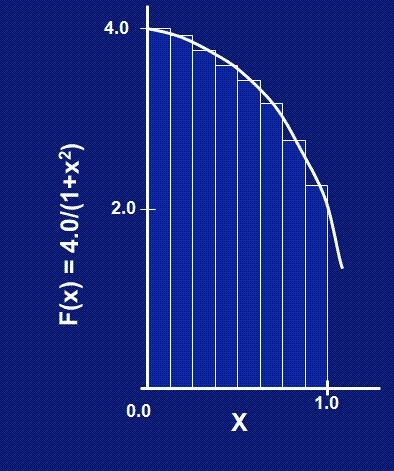
\includegraphics[width=4cm]{./pi}
    \end{center}
  \end{columns}

  \begin{algorithm}[H]
    \caption{Pseudo Code for Calculating Pi}
    \begin{algorithmic}
        \Function{calculate\_pi}{}
        \State $step \gets 1/n$
        \State $sum \gets 0$
        \Do{$i \gets 0\cdots n$}
        \State $x \gets (i+0.5)*step; sum \gets sum + 4/(1+x^2)$
        \EndDo
        \State $pi \gets sum * step$
        \EndFunction
    \end{algorithmic}
  \end{algorithm}
\end{frame}


\begin{frame}{SAXPY}
  \begin{itemize}
    \item SAXPY is a common operation in computations with vector processors included as part of the BLAS routines
    \item[] $y\leftarrow \alpha x + y$
%    \item SAXPY is a combination of scalar multiplication and vector addition
    \item Write a SAXPY code to multiply a vector with a scalar.
  \end{itemize}
  \begin{algorithm}[H]
    \caption{Pseudo Code for SAXPY}
    \begin{algorithmic}
      \Program{saxpy}{}
      \State $n \gets$ some large number
      \State $x(1:n) \gets$ some number say, 1
      \State $y(1:n) \gets$ some other number say, 2
      \State $a \gets$ some other number ,say, 3
      \Do{$i \gets 1\cdots n$}
      \State $y_i \gets y_i + a * x_i$
      \EndDo
      \EndProgram{saxpy}
    \end{algorithmic}
  \end{algorithm}
\end{frame}

\begin{frame}[allowframebreaks]{Matrix Multiplication}
  \begin{itemize}
    \item Most Computational code involve matrix operations such as matrix multiplication.
    \item Consider a matrix {\bf C} which is a product of two matrices {\bf A} and {\bf B}:
    \item[] Element {\it i,j} of {\bf C} is the dot product of the $i^{th}$ row of {\bf A} and $j^{th}$ column of {\bf B}
    \item Write a MATMUL code to multiple two matrices.
  \end{itemize}
  \begin{center}
    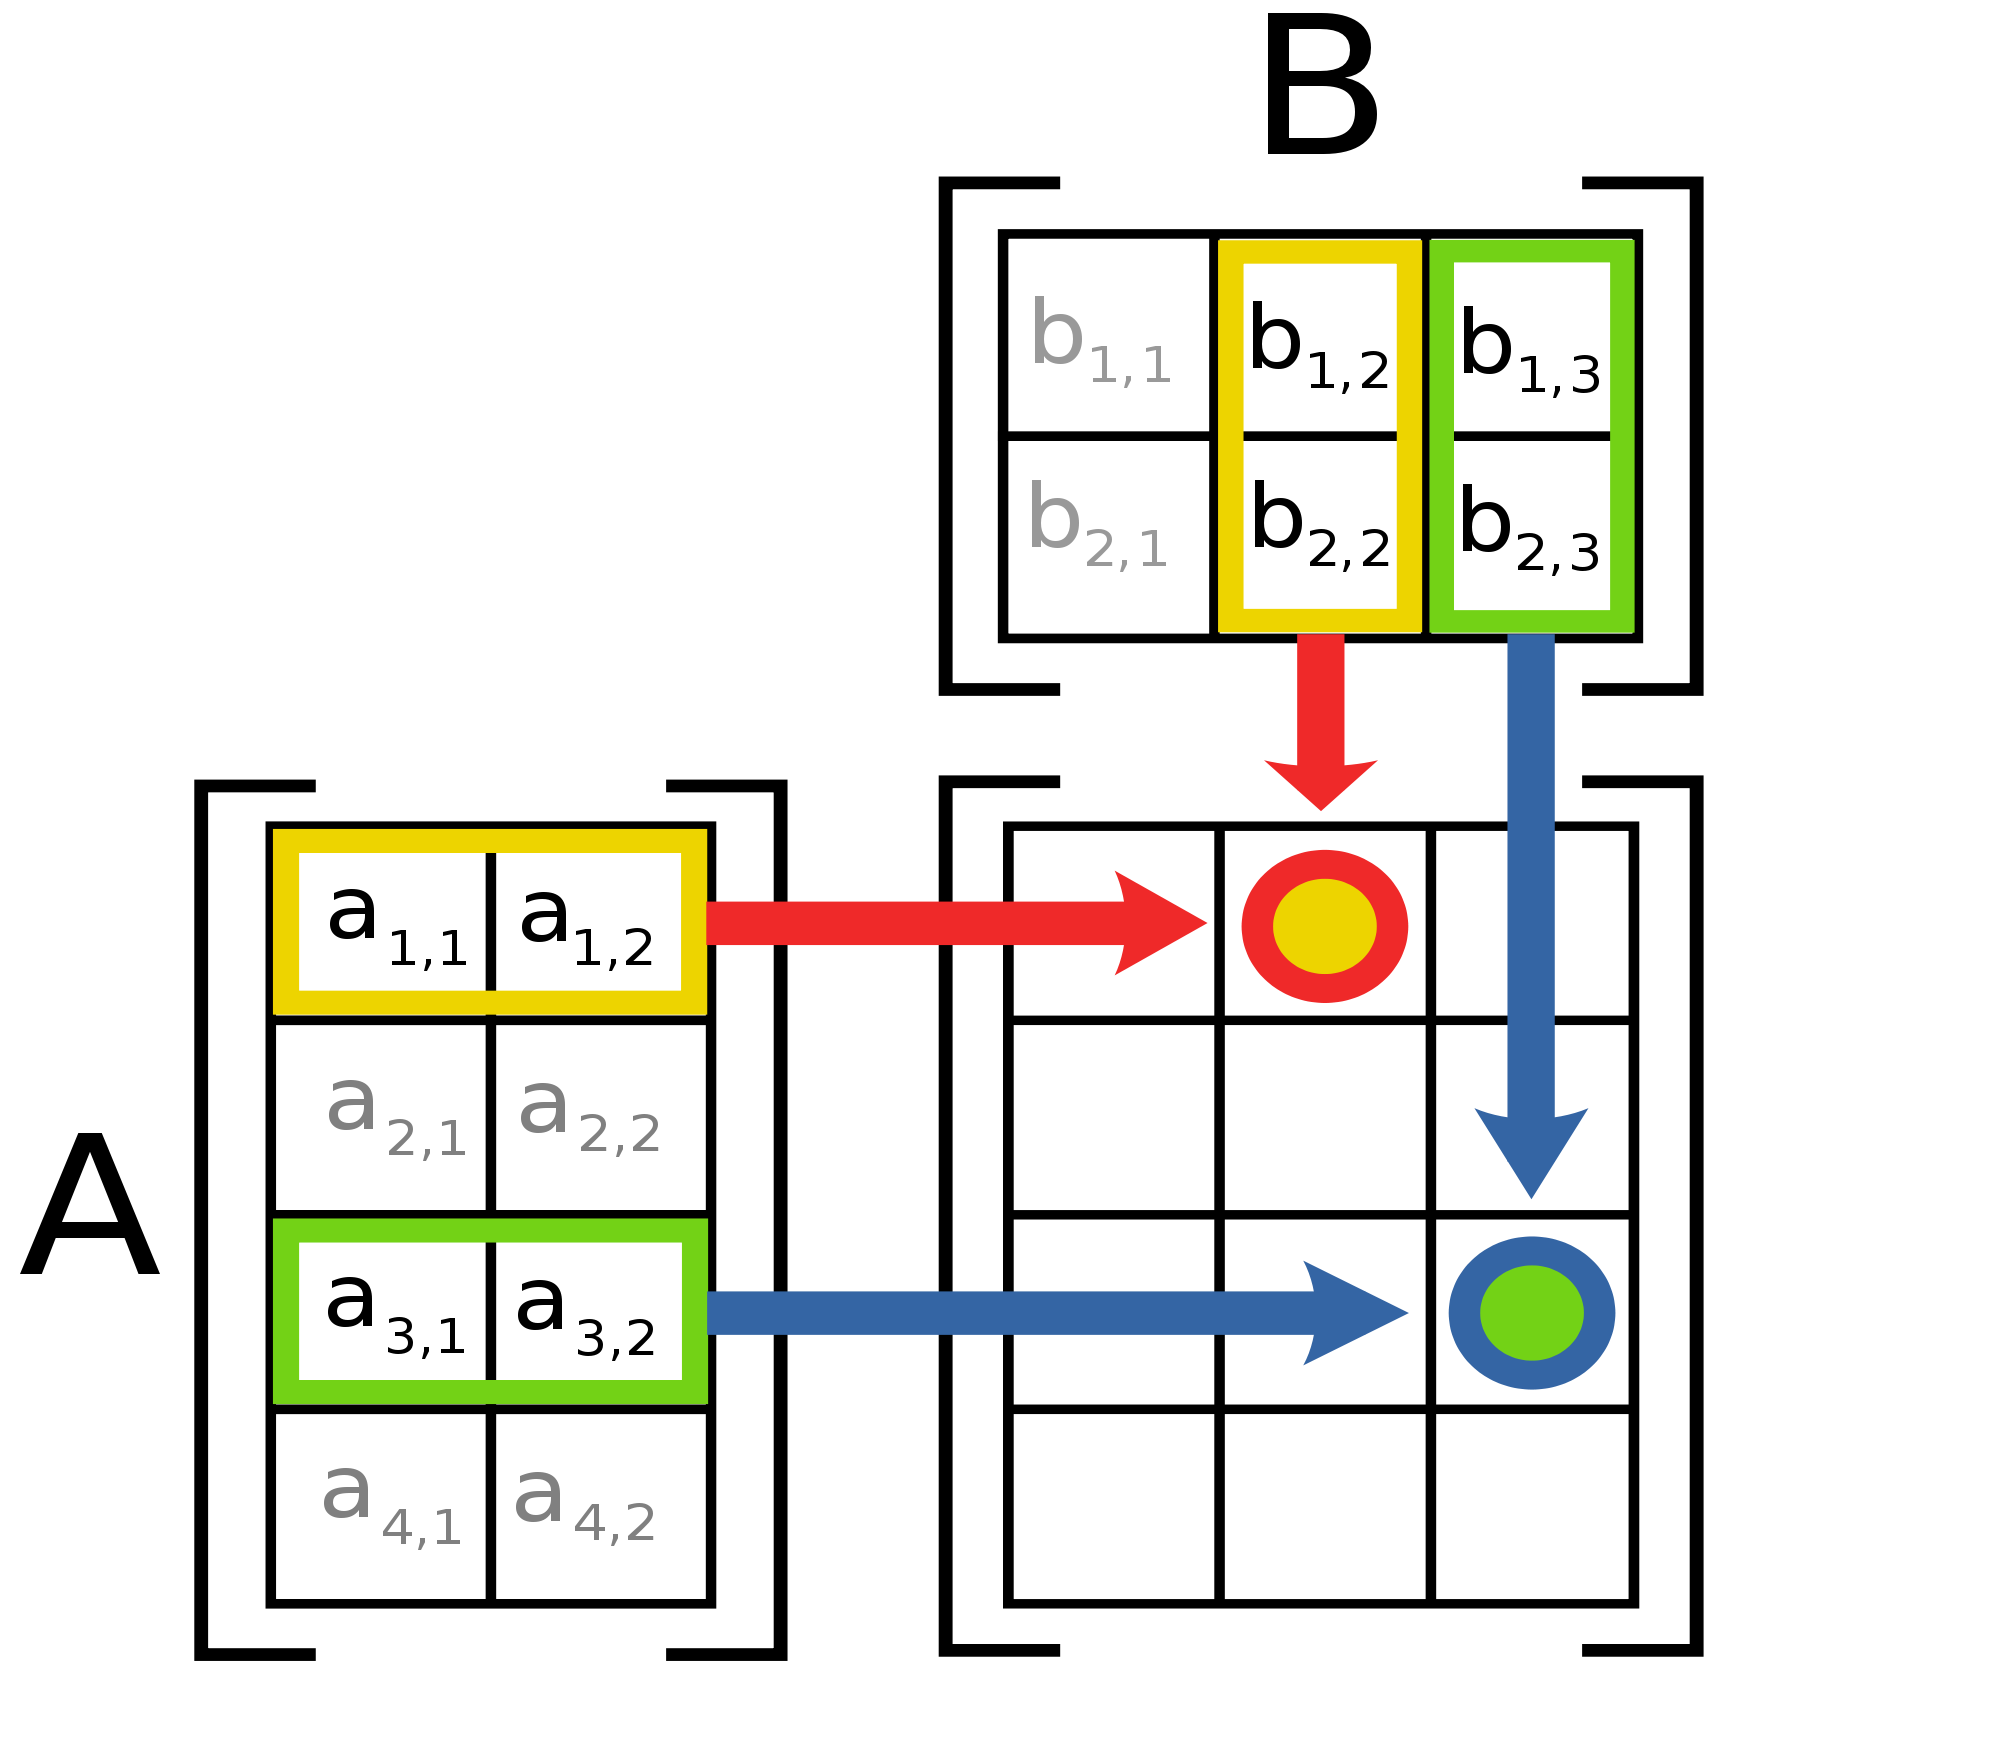
\includegraphics[width=0.3\textwidth]{./matmul}
  \end{center}

  \begin{algorithm}[H]
    \caption{Pseudo Code for MATMUL}
    \begin{algorithmic}
      \Program{matmul}{}
      \State $m,n \gets$ some\,large\,number $\le 1000$
      \State Define $a_{mn}, b_{nm}, c_{mm}$
      \State $a_{ij} \gets i+j; b_{ij} \gets i-j; c_{ij} \gets 0$
      \Do{$i \gets 1\cdots m$}
      \Do{$j \gets 1\cdots m$}
      \State $c_{i,j} \gets \sum^{n}_{k=1} a_{i,k}*b_{k,j}$
      \EndDo
      \EndDo
      \EndProgram{matmul}
    \end{algorithmic}
  \end{algorithm}
\end{frame}

\end{document}



\section{Exercises}
\begin{frame}{Exercise}
  \begin{enumerate}
    \item Print list of prime numbers less than 100
    \item Calculate circumference and area of a circle for given radius
    \item Calculation the Fibonacci sequence of numbers
    \item Calculate factorial of a number
    \item Calculate the Greatest Common Divisor and Least Common Multiple between two integers
  \end{enumerate}
\end{frame}

\end{document}

